\documentclass{article}\usepackage{amsmath,amssymb,amsthm,tikz,tkz-graph,color,chngpage,soul,hyperref,csquotes,graphicx,floatrow}\newcommand*{\QEDB}{\hfill\ensuremath{\square}}\newtheorem*{prop}{Proposition}\renewcommand{\theenumi}{\alph{enumi}}\usepackage[shortlabels]{enumitem}\usepackage[nobreak=true]{mdframed}\usetikzlibrary{matrix,calc}\MakeOuterQuote{"}\usepackage[margin=0.75in]{geometry} \newtheorem{theorem}{Theorem}

\title{EE16A - Lecture 12 Notes}
\author{Name: Felix Su$\quad$SID: 25794773}
\date{Spring 2016$\quad$GSI: Ena Hariyoshi}
\begin{document}
\maketitle

%%%% Topic %%%%
\subsection*{Power}
%%%% Notes %%%%
\begin{itemize}
\item Energy disappated over time: $P = \frac{Energy}{Time}$
\end{itemize}
\begin{mdframed}
\textbf{Power Equations:}\\
\begin{equation}P = VI = I^2R=\frac{V^2}{R}\end{equation}
\end{mdframed}

%%%% Topic %%%%
\subsection*{Thevenin's Equivalence}
%%%% Notes %%%%
\begin{center}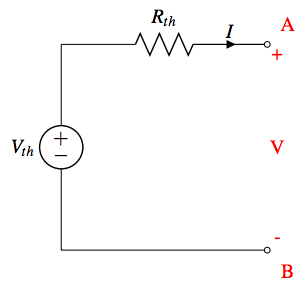
\includegraphics{thev}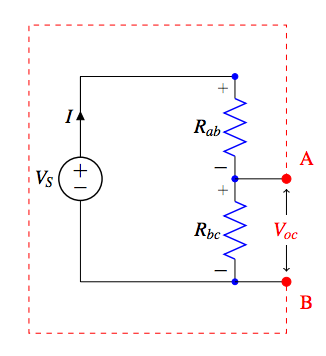
\includegraphics{th_voc}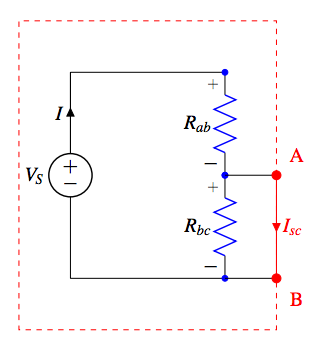
\includegraphics{th_isc}\end{center}
\begin{itemize}
\item Open Circuit: Find voltage drop between two nodes in normal circuit ($V_{oc}$). No current is flowing (no voltage drop over resistor).
\item Short Circuit: Find current between two nodes, skip everything between them ($I_{sc}$)
\end{itemize}
\begin{mdframed}
\textbf{Thevenin Equations:}\\
\begin{equation}V_{th} = V_{oc}\end{equation}
\begin{equation}R_{th} = \frac{V_{th}}{I_{sc}}\end{equation}
\end{mdframed}
\end{document}